

% Options for packages loaded elsewhere
\PassOptionsToPackage{unicode}{hyperref}
\PassOptionsToPackage{hyphens}{url}
%
\documentclass[
  man]{apa6}
\usepackage{lmodern}
\usepackage{amssymb,amsmath}
\usepackage{ifxetex,ifluatex}
\ifnum 0\ifxetex 1\fi\ifluatex 1\fi=0 % if pdftex
  \usepackage[T1]{fontenc}
  \usepackage[utf8]{inputenc}
  \usepackage{textcomp} % provide euro and other symbols
\else % if luatex or xetex
  \usepackage{unicode-math}
  \defaultfontfeatures{Scale=MatchLowercase}
  \defaultfontfeatures[\rmfamily]{Ligatures=TeX,Scale=1}
\fi
% Use upquote if available, for straight quotes in verbatim environments
\IfFileExists{upquote.sty}{\usepackage{upquote}}{}
\IfFileExists{microtype.sty}{% use microtype if available
  \usepackage[]{microtype}
  \UseMicrotypeSet[protrusion]{basicmath} % disable protrusion for tt fonts
}{}
\makeatletter
\@ifundefined{KOMAClassName}{% if non-KOMA class
  \IfFileExists{parskip.sty}{%
    \usepackage{parskip}
  }{% else
    \setlength{\parindent}{0pt}
    \setlength{\parskip}{6pt plus 2pt minus 1pt}}
}{% if KOMA class
  \KOMAoptions{parskip=half}}
\makeatother
\usepackage{xcolor}
\IfFileExists{xurl.sty}{\usepackage{xurl}}{} % add URL line breaks if available
\IfFileExists{bookmark.sty}{\usepackage{bookmark}}{\usepackage{hyperref}}
\hypersetup{
  pdftitle={Theoretical Bias and variance, as a function of population parameters},
  pdfauthor={Delacre Marie},
  pdfkeywords={keywords},
  hidelinks,
  pdfcreator={LaTeX via pandoc}}
\urlstyle{same} % disable monospaced font for URLs
\usepackage{graphicx,grffile}
\makeatletter
\def\maxwidth{\ifdim\Gin@nat@width>\linewidth\linewidth\else\Gin@nat@width\fi}
\def\maxheight{\ifdim\Gin@nat@height>\textheight\textheight\else\Gin@nat@height\fi}
\makeatother
% Scale images if necessary, so that they will not overflow the page
% margins by default, and it is still possible to overwrite the defaults
% using explicit options in \includegraphics[width, height, ...]{}
\setkeys{Gin}{width=\maxwidth,height=\maxheight,keepaspectratio}
% Set default figure placement to htbp
\makeatletter
\def\fps@figure{htbp}
\makeatother
\setlength{\emergencystretch}{3em} % prevent overfull lines
\providecommand{\tightlist}{%
  \setlength{\itemsep}{0pt}\setlength{\parskip}{0pt}}
\setcounter{secnumdepth}{-\maxdimen} % remove section numbering
\shorttitle{Theoretical Bias and variance}
\affiliation{
\vspace{0.5cm}
\textsuperscript{1} ULB}
\keywords{keywords\newline\indent Word count: X}
\usepackage{csquotes}
\usepackage{upgreek}
\captionsetup{font=singlespacing,justification=justified}

\usepackage{longtable}
\usepackage{lscape}
\usepackage{multirow}
\usepackage{tabularx}
\usepackage[flushleft]{threeparttable}
\usepackage{threeparttablex}

\newenvironment{lltable}{\begin{landscape}\begin{center}\begin{ThreePartTable}}{\end{ThreePartTable}\end{center}\end{landscape}}

\makeatletter
\newcommand\LastLTentrywidth{1em}
\newlength\longtablewidth
\setlength{\longtablewidth}{1in}
\newcommand{\getlongtablewidth}{\begingroup \ifcsname LT@\roman{LT@tables}\endcsname \global\longtablewidth=0pt \renewcommand{\LT@entry}[2]{\global\advance\longtablewidth by ##2\relax\gdef\LastLTentrywidth{##2}}\@nameuse{LT@\roman{LT@tables}} \fi \endgroup}


\DeclareDelayedFloatFlavor{ThreePartTable}{table}
\DeclareDelayedFloatFlavor{lltable}{table}
\DeclareDelayedFloatFlavor*{longtable}{table}
\makeatletter
\renewcommand{\efloat@iwrite}[1]{\immediate\expandafter\protected@write\csname efloat@post#1\endcsname{}}
\makeatother
\usepackage{lineno}

\linenumbers

\title{Theoretical Bias and variance, as a function of population parameters}
\author{Delacre Marie\textsuperscript{1}}
\date{}

\begin{document}
\maketitle

\hypertarget{the-bias}{%
\section{The bias}\label{the-bias}}

For all estimators, when the population effect size is null so is the bias. We will subdivise all configurations when there is a non-null population effect into 3 conditions:\\
- when variances are equal across groups,\\
- when variances are unequal across groups, with equal sample sizes\\
- when variances are unequal across groups, with unequal sample sizes

\hypertarget{cohens-d_s}{%
\subsection{\texorpdfstring{Cohen's \(d_s\)}{Cohen's d\_s}}\label{cohens-d_s}}

\hypertarget{when-variances-are-equal-across-populations}{%
\subsubsection{When variances are equal across populations}\label{when-variances-are-equal-across-populations}}

The \textbf{bias} of Cohen's \(d_s\) is a function of total sample size (N) and the population effect size (\(\delta_{Cohen}\)):

\begin{itemize}
\tightlist
\item
  The larger the population effect size, the more Cohen's \(d_s\) will overestimate \(\delta_{Cohen}\).
\end{itemize}

\begin{figure}
\centering
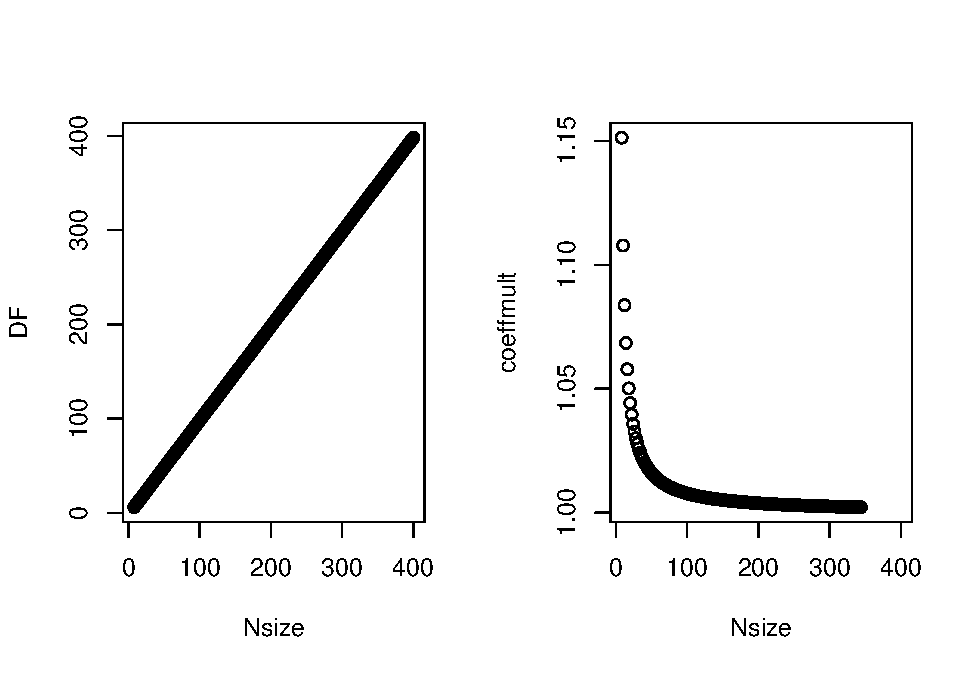
\includegraphics{Theoretical-Bias-of-all-estimators-as-a-function-of-population-parameters_files/figure-latex/biascohendNsize2-1.pdf}
\caption{\label{fig:biascohendNsize2}\ldots{}}
\end{figure}

\begin{itemize}
\tightlist
\item
  The larger the total sample size, the lower the bias. The bias tends to zero when the total sample size tends to infinity (see Figure \ref{fig:biascohendNsize2})
\end{itemize}

\begin{figure}
\centering
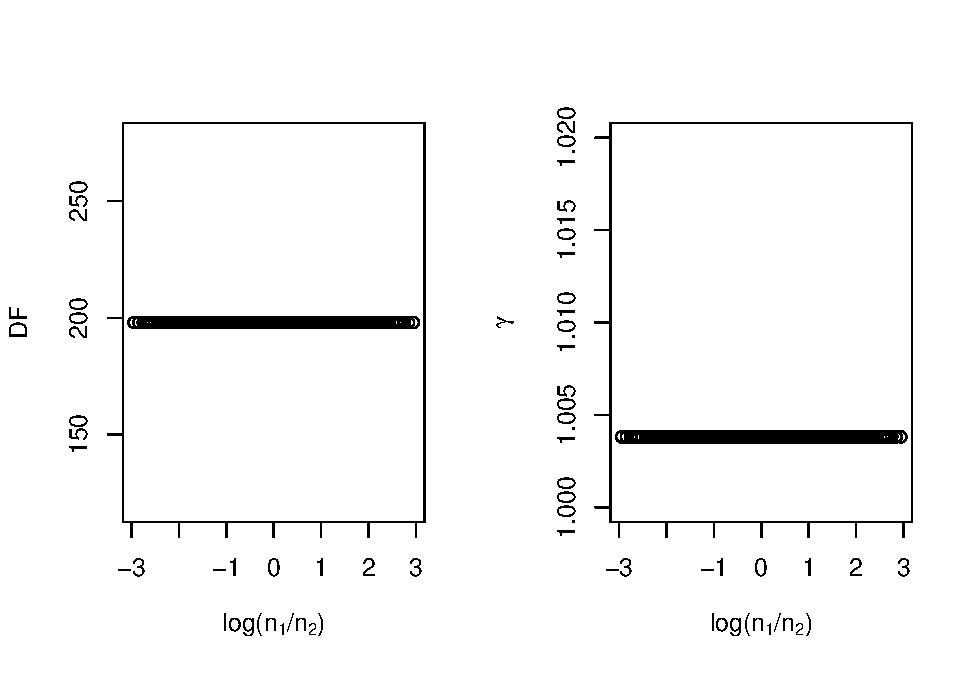
\includegraphics{Theoretical-Bias-of-all-estimators-as-a-function-of-population-parameters_files/figure-latex/biascohendNratio2-1.pdf}
\caption{\label{fig:biascohendNratio2}\ldots{}}
\end{figure}

Of course, considering the degrees of freedom, the sample size ratio does not matter\ldots(see Figure \ref{fig:biascohendNratio2})

\hypertarget{glasss-d_s}{%
\subsection{\texorpdfstring{Glass's \(d_s\)}{Glass's d\_s}}\label{glasss-d_s}}

Because degrees of freedom depend only on the sample size of the control group, there is no need to distinguish between cases where there is homoscedasticity or heteroscedasticity!

The \textbf{bias} of Glass's \(d_s\) is a function of the sample size of the control group (\(n_c\)) and the population effect size (\(\delta_{glass}\)):

\begin{itemize}
\tightlist
\item
  The larger the population effect size, the more Glass's \(d_s\) will overestimate \(\delta_{Glass}\).
\end{itemize}

\begin{figure}
\centering
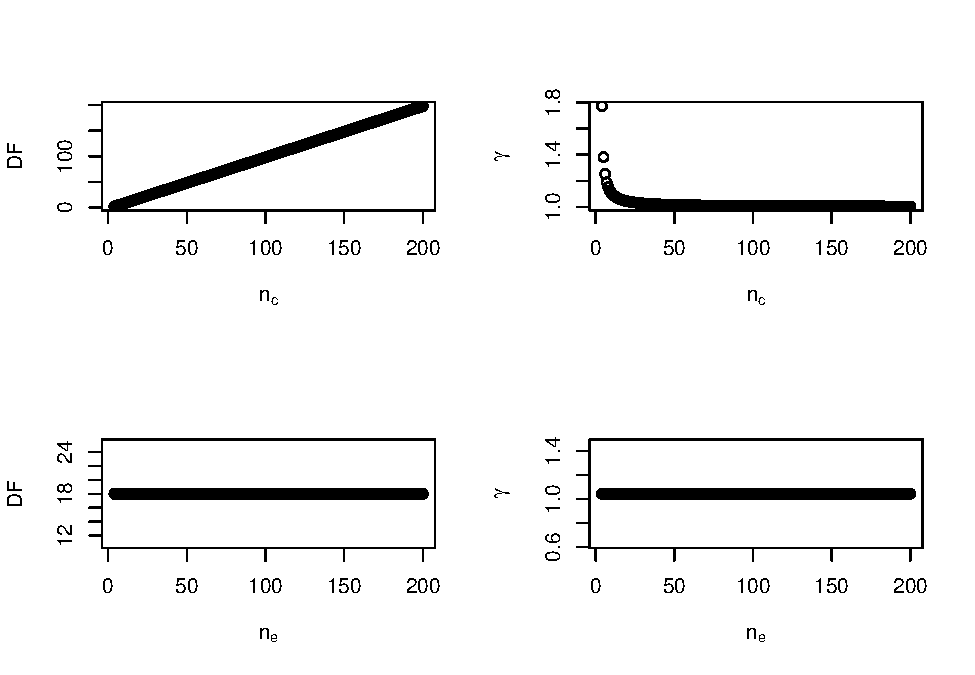
\includegraphics{Theoretical-Bias-of-all-estimators-as-a-function-of-population-parameters_files/figure-latex/biasGlassctrlsize2-1.pdf}
\caption{\label{fig:biasGlassctrlsize2}\ldots{}}
\end{figure}

\begin{itemize}
\tightlist
\item
  The larger the size of the control group, the lower the bias. The bias tends to zero when the sample size of the control group tends to infinity (see Figure \ref{fig:biasGlassctrlsize2})
\end{itemize}

\hypertarget{cohens-d_s-1}{%
\subsection{\texorpdfstring{Cohen's \(d'_s\)}{Cohen's d'\_s}}\label{cohens-d_s-1}}

\hypertarget{when-variances-are-equal-across-populations-1}{%
\subsubsection{When variances are equal across populations}\label{when-variances-are-equal-across-populations-1}}

When \(\sigma_1=\sigma_2=\sigma\):
\[df_{Cohen's \; d'_s} = \frac{(n_1-1)(n_2-1)(2\sigma^2)^2}{(n_2-1)\sigma^4+(n_1-1)\sigma^4} = \frac{(n_1-1)(n_2-1)\times 4\sigma^4}{\sigma^4(n_1+n_2-2)} = \frac{4(n_1-1)(n_2-1)}{n_1+n_2-2}\]
One can see that degrees of freedom depend only on the total sample size (N) and the sample size allocation ratio. As a consequence, the \textbf{bias} of Cohen's \(d'_s\) is a function of the population effect size (\(\delta'_{Cohen}\)), the sample size allocation ratio and the total sample size (\(N\)).

\begin{itemize}
\tightlist
\item
  The larger the population effect size, the more \(Cohen's \; d'_s\) will overestimate \(\delta'_{Cohen}\)
\end{itemize}

\begin{figure}
\centering
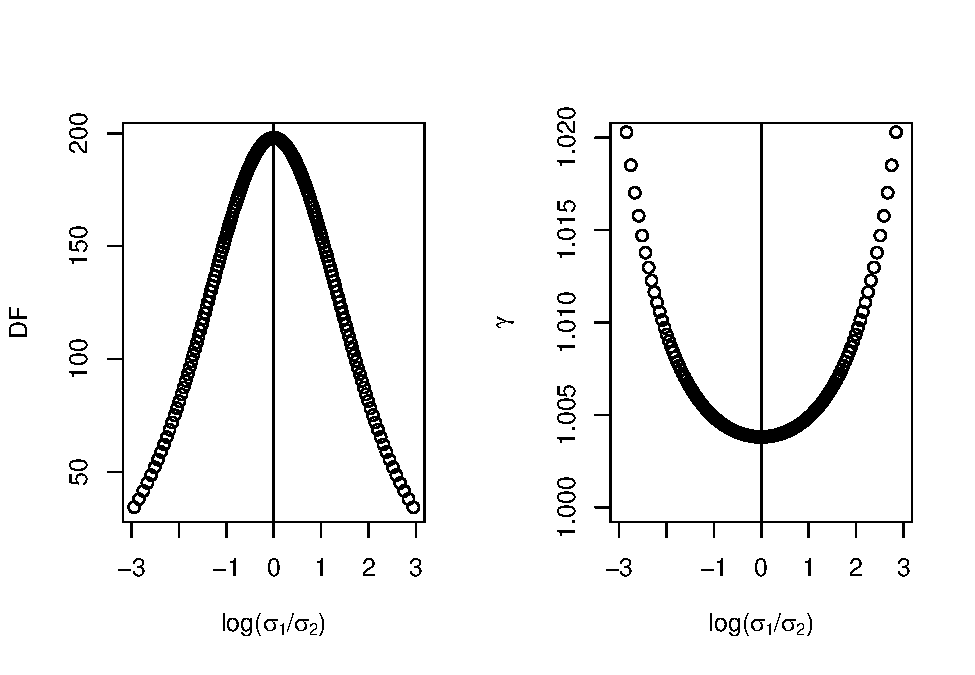
\includegraphics{Theoretical-Bias-of-all-estimators-as-a-function-of-population-parameters_files/figure-latex/biascohendprimehomNratio2-1.pdf}
\caption{\label{fig:biascohendprimehomNratio2}\ldots{}}
\end{figure}

\begin{itemize}
\tightlist
\item
  The further the sample size allocation ratio is from 1, the larger the bias (see Figure \ref{fig:biascohendprimehomNratio2})
\end{itemize}

\begin{figure}
\centering
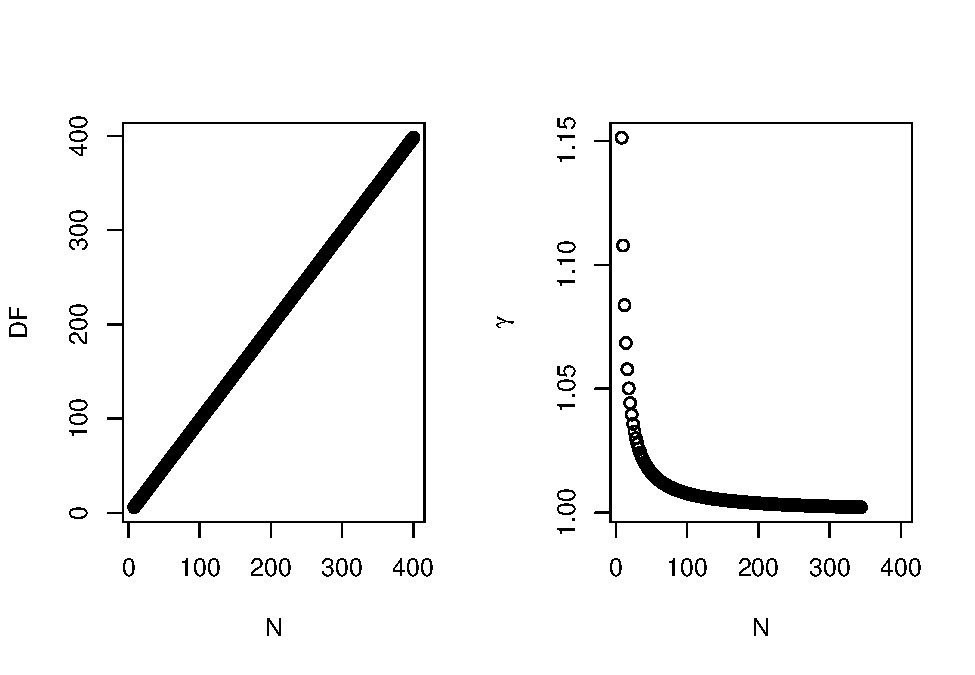
\includegraphics{Theoretical-Bias-of-all-estimators-as-a-function-of-population-parameters_files/figure-latex/biascohendprimehomNsize2-1.pdf}
\caption{\label{fig:biascohendprimehomNsize2}\ldots{}}
\end{figure}

\begin{itemize}
\tightlist
\item
  The larger the total sample size, the lower the bias (see Figure \ref{fig:biascohendprimehomNsize2})
\end{itemize}

\hypertarget{when-variances-are-unequal-across-populations-with-equal-sample-sizes}{%
\subsubsection{When variances are unequal across populations, with equal sample sizes}\label{when-variances-are-unequal-across-populations-with-equal-sample-sizes}}

When \(n_1=n_2=n\):
\[df_{Cohen's \; d'_s} = \frac{(n-1)^2(\sigma^2_1+\sigma^2_2)^2}{(n-1)(\sigma^4_1+\sigma^4_2)} =  \frac{(n-1)(\sigma^4_1+\sigma^4_2+2\sigma^2_1\sigma^2_2)}{\sigma^4_1+\sigma^4_2}\]
One can see that degrees of freedom depend only on the total sample size (N) and the SD-ratio. As a consequence, the \textbf{bias} of Cohen's \(d'_s\) is a function of the population effect size (\(\delta'_{Cohen}\)), the SD-ratio and the total sample size (\(N\)):

\begin{itemize}
\tightlist
\item
  The larger the population effect size, the more \(Cohen's \; d'_s\) will overestimate \(\delta'_{Cohen}\)
\end{itemize}

\begin{figure}
\centering
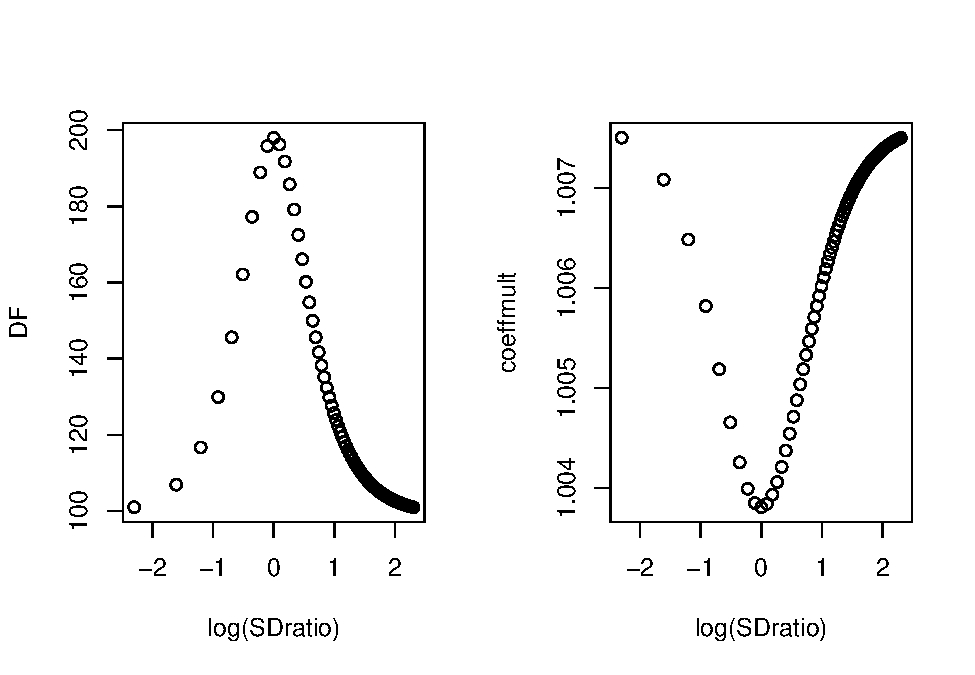
\includegraphics{Theoretical-Bias-of-all-estimators-as-a-function-of-population-parameters_files/figure-latex/biascohendprimehetbalSDratio2-1.pdf}
\caption{\label{fig:biascohendprimehetbalSDratio2}\ldots{}}
\end{figure}

\begin{itemize}
\tightlist
\item
  The further the SD-ratio is from 1, the larger the bias (see Figure \ref{fig:biascohendprimehetbalSDratio2})
\end{itemize}

\begin{figure}
\centering
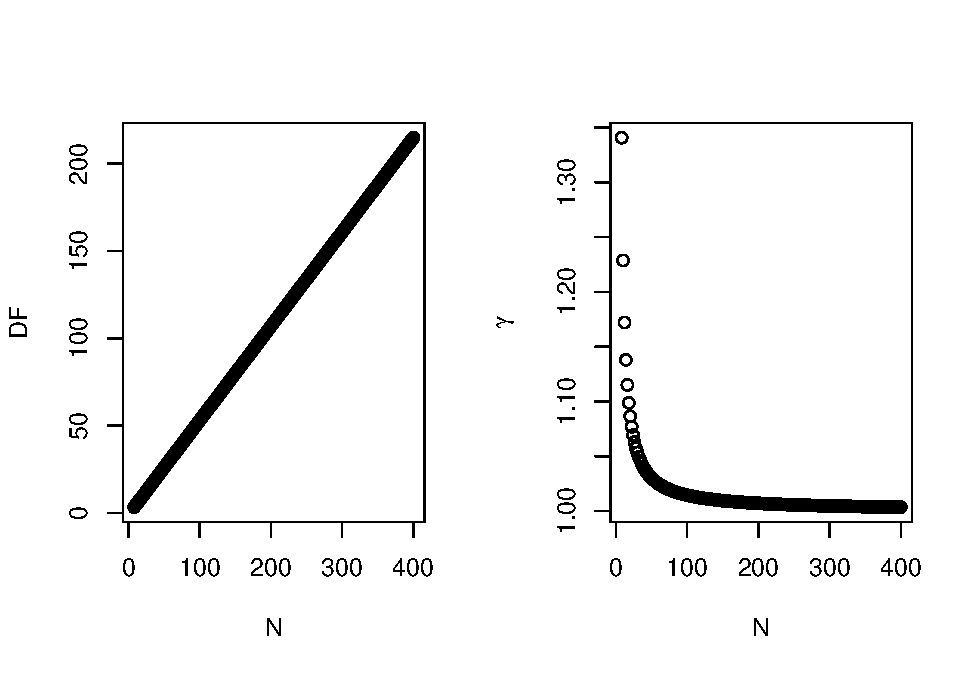
\includegraphics{Theoretical-Bias-of-all-estimators-as-a-function-of-population-parameters_files/figure-latex/biascohendprimehetbalNsize2-1.pdf}
\caption{\label{fig:biascohendprimehetbalNsize2}\ldots{}}
\end{figure}

\begin{itemize}
\tightlist
\item
  The larger the total sample size, the lower the bias (see Figure \ref{fig:biascohendprimehetbalNsize2})
\end{itemize}

\begin{figure}
\centering
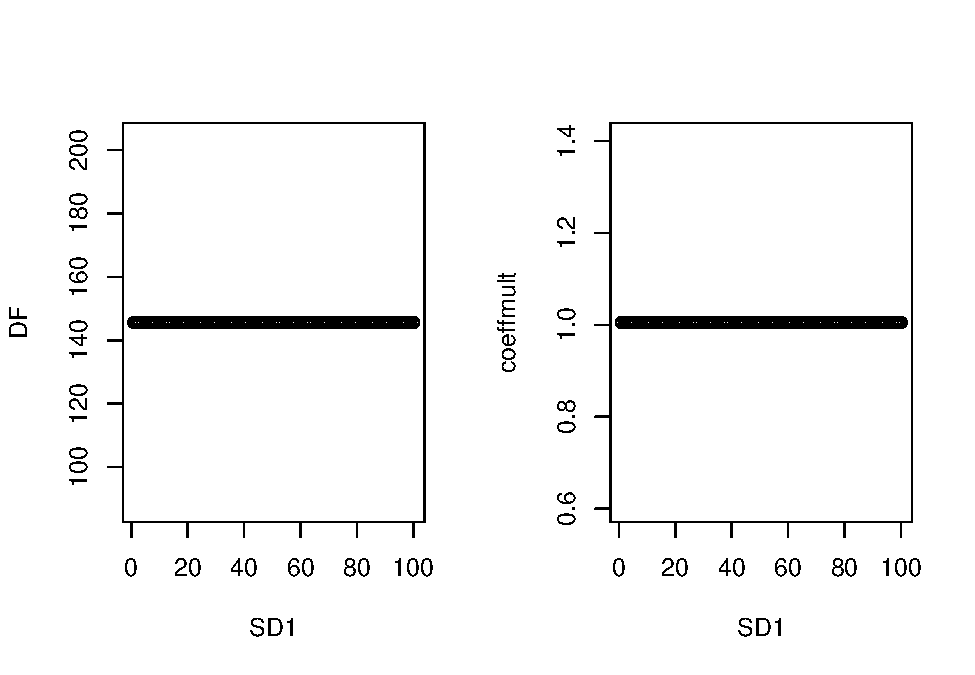
\includegraphics{Theoretical-Bias-of-all-estimators-as-a-function-of-population-parameters_files/figure-latex/biascohendprimehetbalvariance2-1.pdf}
\caption{\label{fig:biascohendprimehetbalvariance2}\ldots{}}
\end{figure}

Note: for a constant SD-ratio, the size of the variance does not matter (see Figure \ref{fig:biascohendprimehetbalvariance2})

\hypertarget{when-variances-are-unequal-across-populations-with-unequal-sample-sizes}{%
\subsubsection{When variances are unequal across populations, with unequal sample sizes}\label{when-variances-are-unequal-across-populations-with-unequal-sample-sizes}}

The \textbf{bias} of Cohen's \(d'_s\) is a function of the population effect size (\(\delta'_{Cohen}\)), the total sample size, and the sample sizes and variances pairing :

\begin{itemize}
\tightlist
\item
  The larger the population effect size, the more \(Cohen's \; d'_s\) will overestimate \(\delta'_{Cohen}\)
\end{itemize}

\begin{figure}
\centering
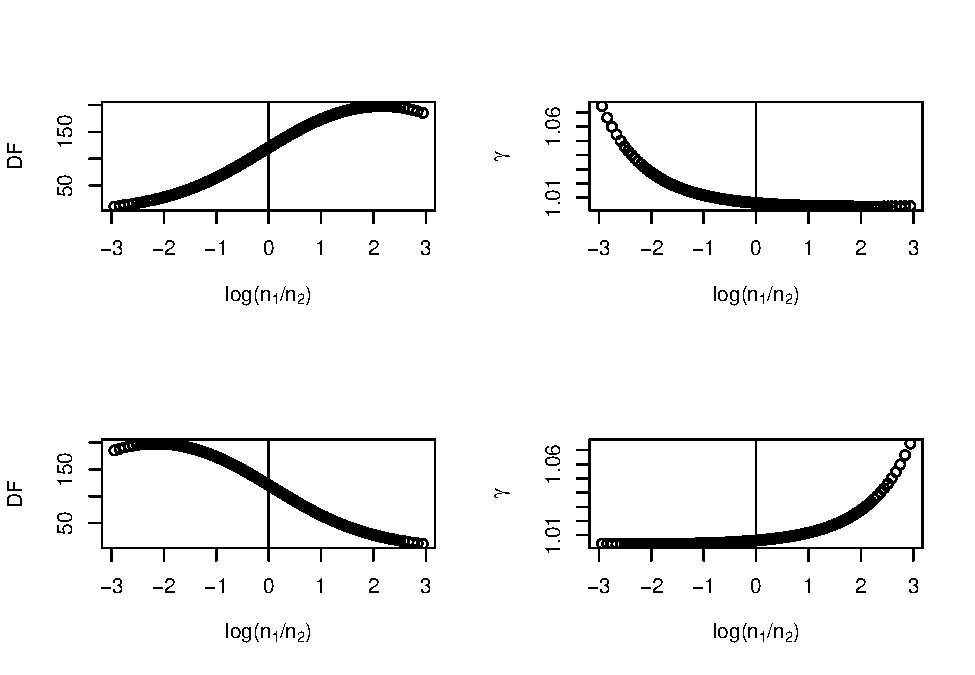
\includegraphics{Theoretical-Bias-of-all-estimators-as-a-function-of-population-parameters_files/figure-latex/biascohendprimehetunbalNratio2-1.pdf}
\caption{\label{fig:biascohendprimehetunbalNratio2}\ldots{}}
\end{figure}

\begin{itemize}
\tightlist
\item
  When there is a positive pairing between sample sizes and variances, one gives more weight to the smallest variance. As a consequence, the denominator in the df computation decreases, the degrees of freedom increase and therefore, the bias decreases (see the two plots on the top in Figure \ref{fig:biascohendprimehetunbalNratio2}). On the other size, where there is a negative pairing between sample sizes and variances, one gives more weight to the largest variance. As a consequence, the denominator in the df computatin increases, the degrees of freedom decrease and therefore, the bias increase (see the two plots in the bottom of Figure \ref{fig:biascohendprimehetunbalNratio2}).
\end{itemize}

\begin{figure}
\centering
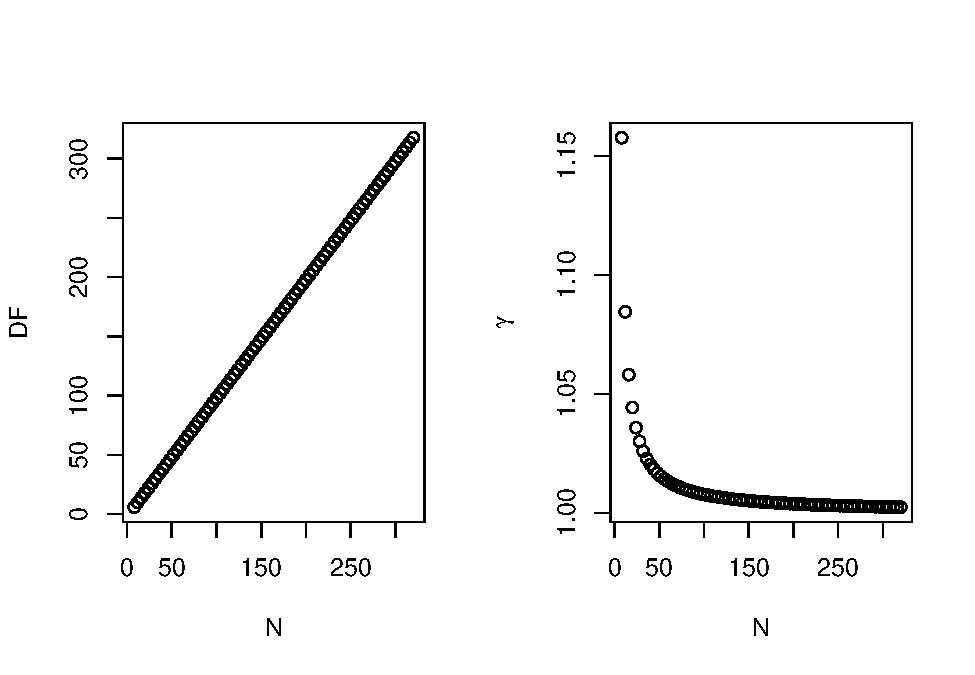
\includegraphics{Theoretical-Bias-of-all-estimators-as-a-function-of-population-parameters_files/figure-latex/biascohendprimehetunbalNsize2-1.pdf}
\caption{\label{fig:biascohendprimehetunbalNsize2}\ldots{}}
\end{figure}

\begin{itemize}
\tightlist
\item
  The larger the total sample size, the lower the bias (illustration in Figure \ref{fig:biascohendprimehetunbalNsize2})
\end{itemize}

\begin{figure}
\centering
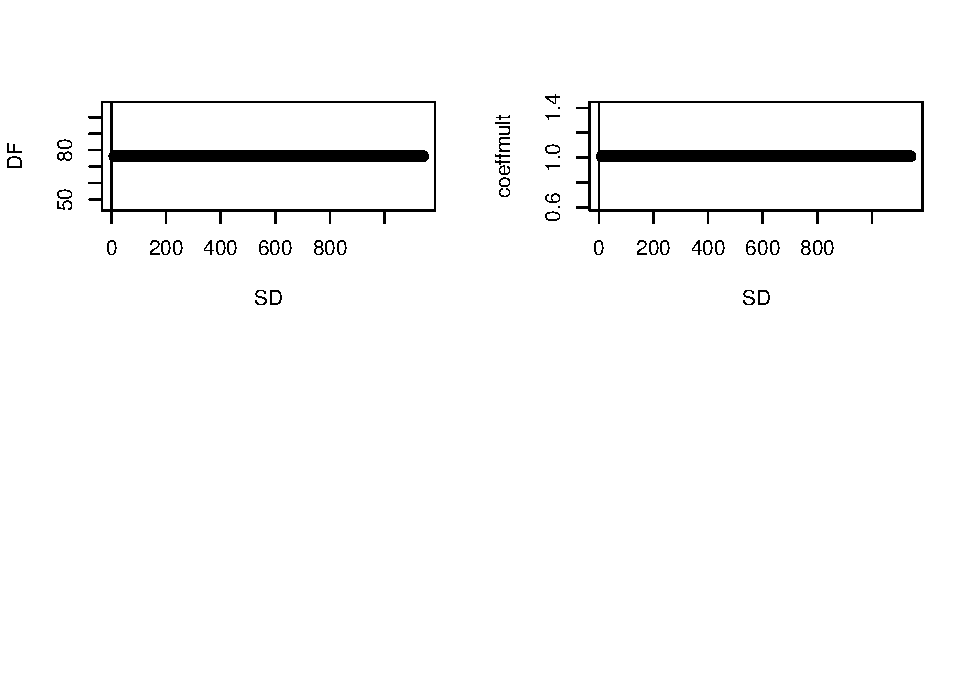
\includegraphics{Theoretical-Bias-of-all-estimators-as-a-function-of-population-parameters_files/figure-latex/biascohendprimehetunbalvariance2-1.pdf}
\caption{\label{fig:biascohendprimehetunbalvariance2}\ldots{}}
\end{figure}

Note: for a constant SD-ratio, the variance does not matter. (See Figure \ref{fig:biascohendprimehetunbalvariance2})

\hypertarget{shiehs-d_s}{%
\subsection{\texorpdfstring{Shieh's \(d_s\)}{Shieh's d\_s}}\label{shiehs-d_s}}

\hypertarget{when-variances-are-equal-across-populations-2}{%
\subsubsection{When variances are equal across populations}\label{when-variances-are-equal-across-populations-2}}

When \(\sigma_1=\sigma_2=\sigma\):
\[df_{Shieh's \; d_s} = \frac{\left( \frac{n_2\sigma^2+n_1\sigma^2}{n_1n_2}\right)^2}{\frac{(n_2-1)\left( \frac{\sigma^2}{n_1}\right)^2+(n_1-1)\left( \frac{\sigma^2}{n_2}\right)^2}{(n_1-1)(n_2-1)}}\]
\[\leftrightarrow df_{Shieh's \; d_s} = \frac{[\sigma^2(n_1+n_2)]^2}{n_1^2n_2^2} \times \frac{(n_1-1)(n_2-1)}{(n_2-1) \times  \frac{\sigma^4}{n_1^2}+(n_1-1) \times \frac{\sigma^4}{n_2^2}}\]
\[\leftrightarrow df_{Shieh's \; d_s} = \frac{\sigma^4N^2}{n_1^2n_2^2} \times \frac{(n_1-1)(n_2-1)}{\sigma^4 \left( \frac{n_2-1}{n^2_1}+\frac{n_1-1}{n^2_2}\right) }\]
\[\leftrightarrow df_{Shieh's \; d_s} = \frac{N^2(n_1-1)(n_2-1)}{n_1^2n_2^2 \left( \frac{n_2^2(n_2-1)+n_1^2(n_1-1)}{n_1^2n_2^2}\right)}\]
\[\leftrightarrow df_{Shieh's \; d_s} = \frac{N^2(n_1-1)(n_2-1)}{n_2^2(n_2-1)+n_1^2(n_1-1)}\]

One can see that degrees of freedom depend only on the total sample size (N) and the sample size allocation ratio. As a consequence, the \textbf{bias} of Shieh's \(d'_s\) is a function of the population effect size (\(\delta_{Shieh}\)), the sample size allocation ratio and the total sample size (\(N\)).

\begin{itemize}
\tightlist
\item
  The larger the population effect size, the more \(Shieh's \; d_s\) will overestimate \(\delta_{Shieh}\)
\end{itemize}

\begin{figure}
\centering
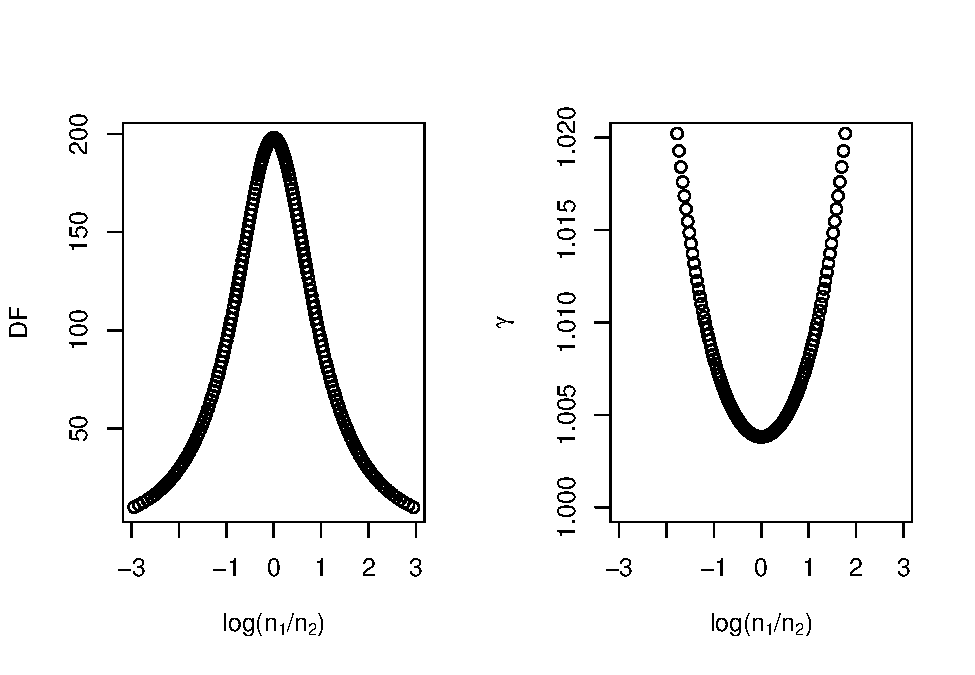
\includegraphics{Theoretical-Bias-of-all-estimators-as-a-function-of-population-parameters_files/figure-latex/biasshiehhomNratio2-1.pdf}
\caption{\label{fig:biasshiehhomNratio2}\ldots{}}
\end{figure}

\begin{itemize}
\tightlist
\item
  The further the sample size allocation ratio is from 1, the larger the bias (see Figure \ref{fig:biasshiehhomNratio2})
\end{itemize}

\begin{figure}
\centering
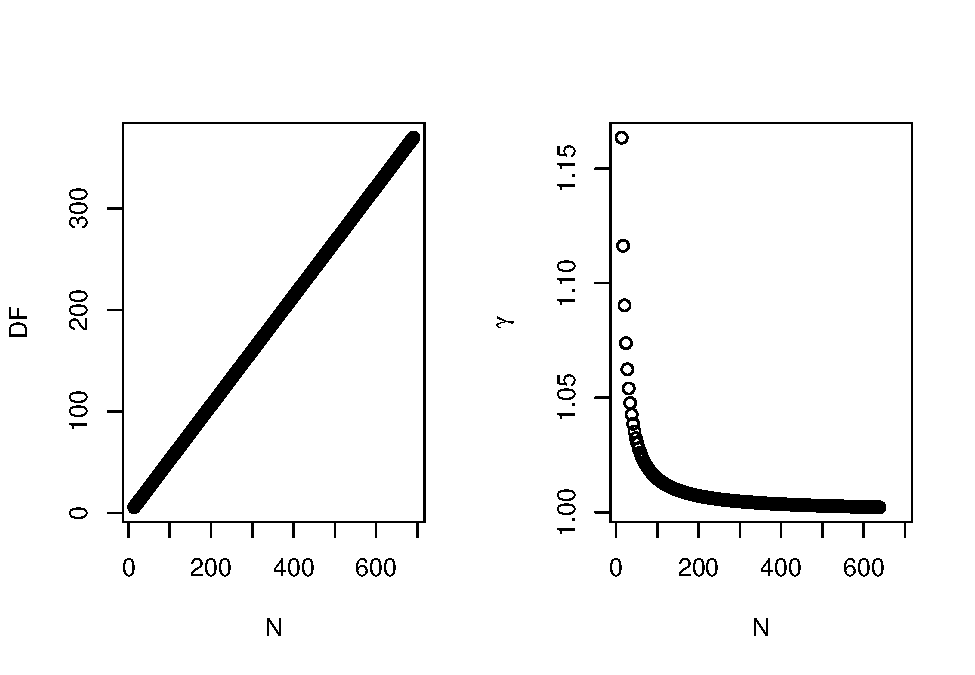
\includegraphics{Theoretical-Bias-of-all-estimators-as-a-function-of-population-parameters_files/figure-latex/biasshiehhomNsize2-1.pdf}
\caption{\label{fig:biasshiehhomNsize2}\ldots{}}
\end{figure}

\begin{itemize}
\tightlist
\item
  The larger the total sample size, the lower the bias (see Figure \ref{fig:biasshiehhomNsize2})
\end{itemize}

\hypertarget{when-variances-are-unequal-across-populations-with-equal-sample-sizes-1}{%
\subsubsection{When variances are unequal across populations, with equal sample sizes}\label{when-variances-are-unequal-across-populations-with-equal-sample-sizes-1}}

When \(n_1=n_2=n\):
\[df_{Shieh's \; d_s} = \frac{\left( \frac{\sigma_1^2+\sigma_2^2}{n} \right)^2}{\frac{(\sigma_1^2/n)^2+(\sigma_2^2/n)^2}{n-1}}\]
\[df_{Shieh's \; d_s} = \frac{(\sigma_1^2+\sigma_2^2)^2}{n^2} \times\frac{n-1}{\frac{\sigma_1^4+\sigma_2^4}{n^2}}\]
\[df_{Shieh's \; d_s} = \frac{(\sigma_1^2+\sigma_2^2)^2 \times (n-1)}{\sigma_1^4+\sigma_2^4}\]

One can see that degrees of freedom depend on the total sample size (N), the \(SD\)-ratio. As a consequence, the bias depends on the population effect size (\(\delta_{Shieh}\)), the \(SD\)-ratio and the total sample size (N).

\begin{itemize}
\tightlist
\item
  The larger the population effect size, the more \(Shieh's \; d_s\) will overestimate \(\delta_{Shieh}\)
\end{itemize}

\begin{figure}
\centering
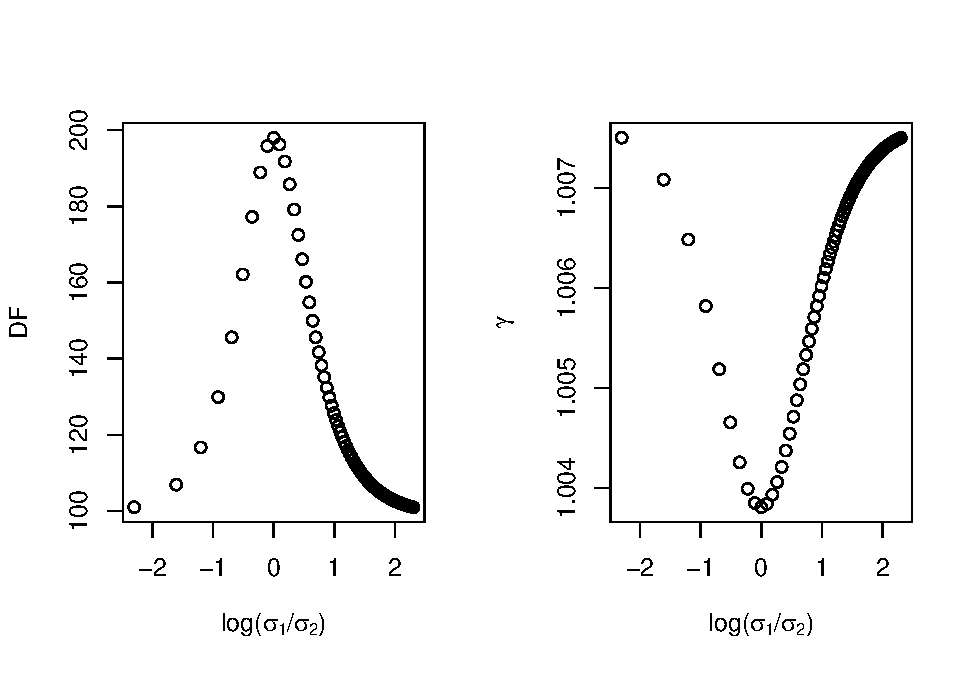
\includegraphics{Theoretical-Bias-of-all-estimators-as-a-function-of-population-parameters_files/figure-latex/biasshiehhetbalSDratio2-1.pdf}
\caption{\label{fig:biasshiehhetbalSDratio2}\ldots{}}
\end{figure}

\begin{itemize}
\tightlist
\item
  The further the SD-ratio is from 1, the larger the bias (see Figure \ref{fig:biasshiehhetbalSDratio2})
\end{itemize}

\begin{figure}
\centering
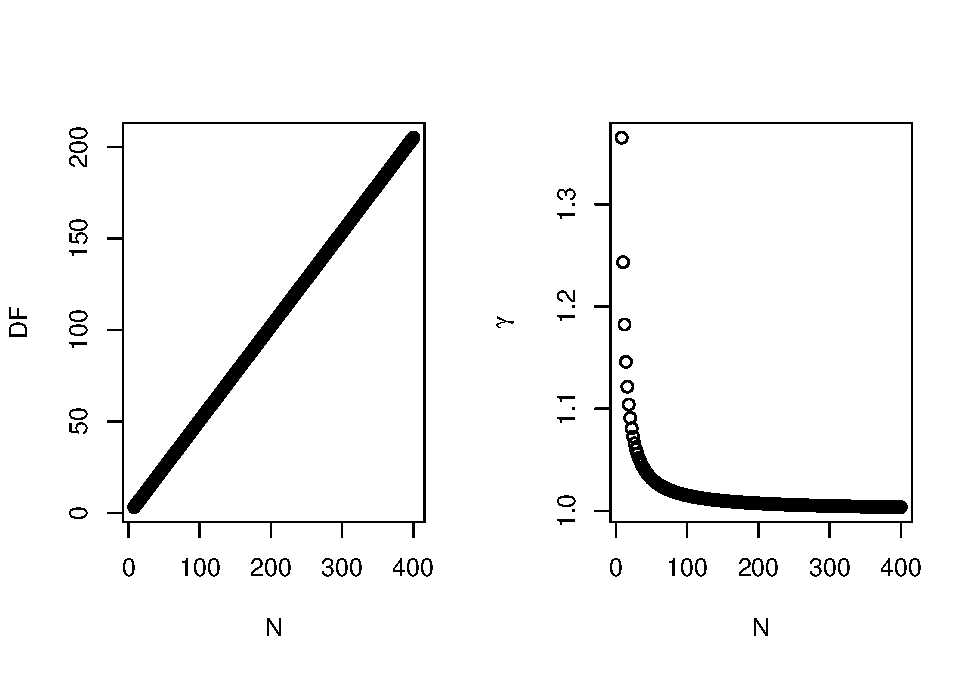
\includegraphics{Theoretical-Bias-of-all-estimators-as-a-function-of-population-parameters_files/figure-latex/biasshiehhetbalNsize2-1.pdf}
\caption{\label{fig:biasshiehhetbalNsize2}bias of Cohen's \(d'_s\) as a function of the total sample size, when variances are equal across groups}
\end{figure}

\begin{itemize}
\tightlist
\item
  The larger the total sample size, the lower the bias (see Figure \ref{fig:biasshiehhetbalNsize2})
\end{itemize}

\begin{figure}
\centering
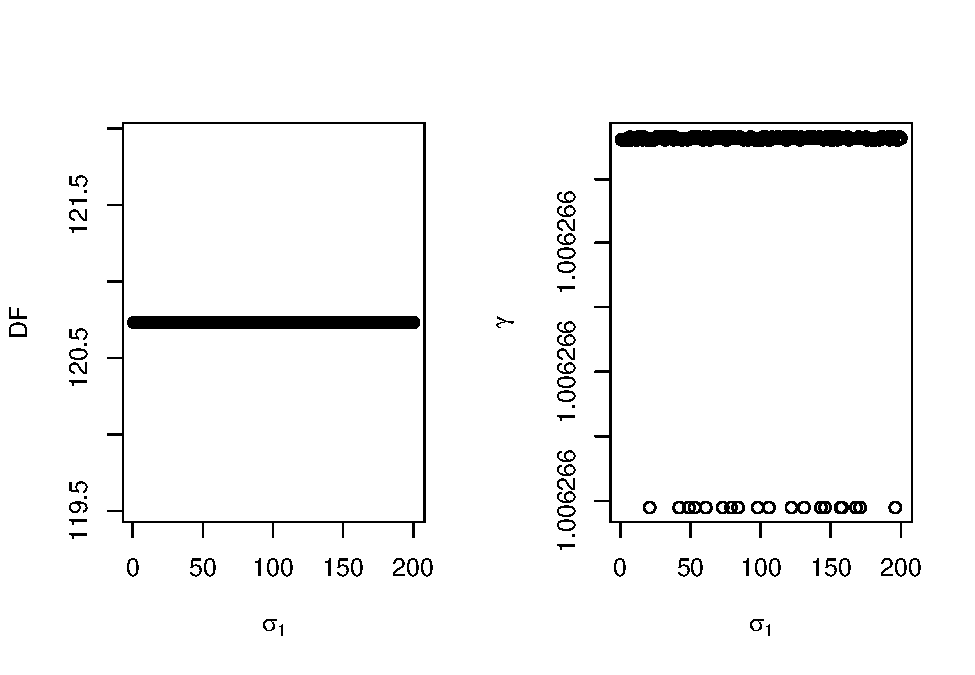
\includegraphics{Theoretical-Bias-of-all-estimators-as-a-function-of-population-parameters_files/figure-latex/biasshiehhetbalvariance2-1.pdf}
\caption{\label{fig:biasshiehhetbalvariance2};;;}
\end{figure}

Note: for a constant SD-ratio, the size of the variance does not matter (see Figure \ref{fig:biasshiehhetbalvariance2})

\hypertarget{when-variances-are-unequal-across-populations-with-unequal-sample-sizes-1}{%
\subsubsection{When variances are unequal across populations, with unequal sample sizes}\label{when-variances-are-unequal-across-populations-with-unequal-sample-sizes-1}}

The \textbf{bias} of Shieh's \(d'_s\) is a function of the population effect size (\(\delta_{Shieh}\)), the sample sizes (\(n_1\) and \(n_2\)), and the pairing between sample sizes and variances and sample sizes ratios.

\begin{itemize}
\tightlist
\item
  The larger the population effect size, the more \(Shieh's \; d_s\) will overestimate \(\delta_{Shieh}\)
\end{itemize}

\begin{figure}
\centering
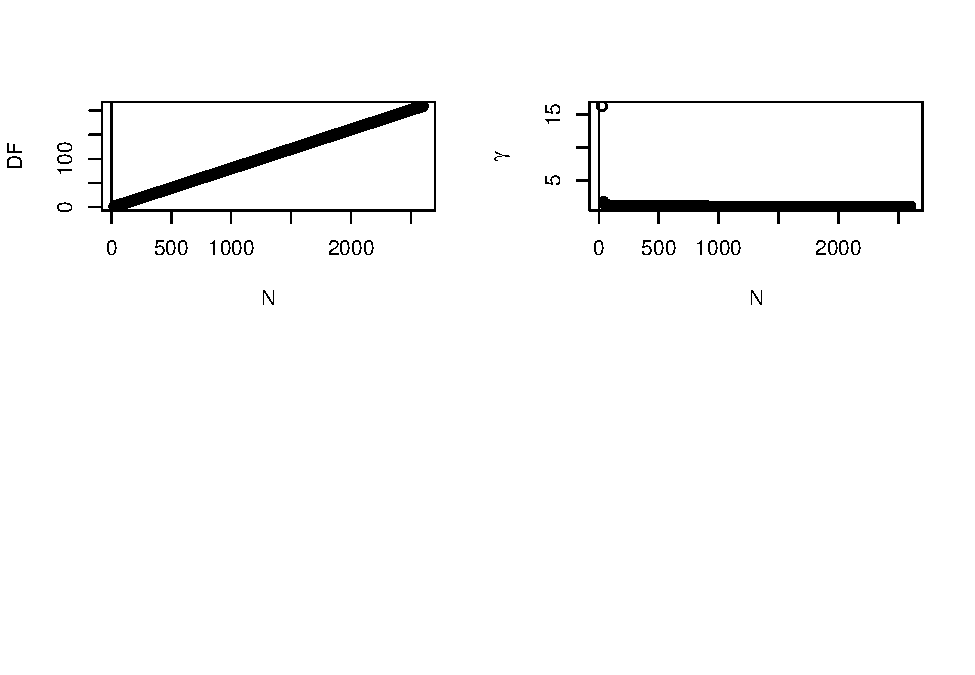
\includegraphics{Theoretical-Bias-of-all-estimators-as-a-function-of-population-parameters_files/figure-latex/biasshiehhetunbalNsize2-1.pdf}
\caption{\label{fig:biasshiehhetunbalNsize2}\ldots{}}
\end{figure}

\begin{itemize}
\tightlist
\item
  The larger the sample sizes, the lower the bias (illustration in Figure \ref{fig:biasshiehhetunbalNsize2})
\end{itemize}

\begin{figure}
\centering
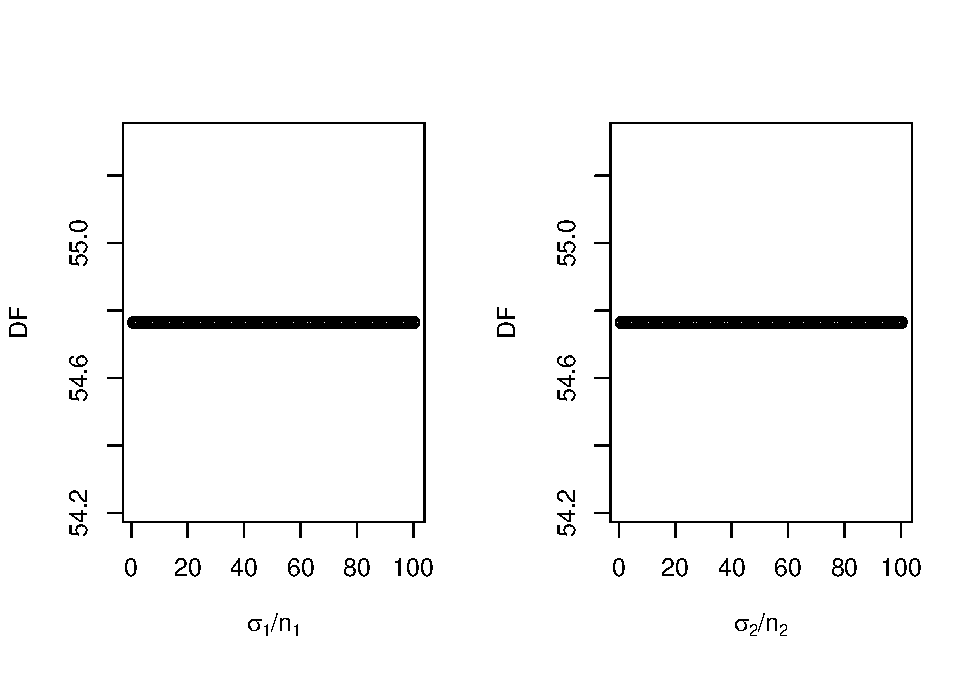
\includegraphics{Theoretical-Bias-of-all-estimators-as-a-function-of-population-parameters_files/figure-latex/biasshiehhetunbalSDRN2-1.pdf}
\caption{\label{fig:biasshiehhetunbalSDRN2}\ldots{}}
\end{figure}

\begin{figure}
\centering
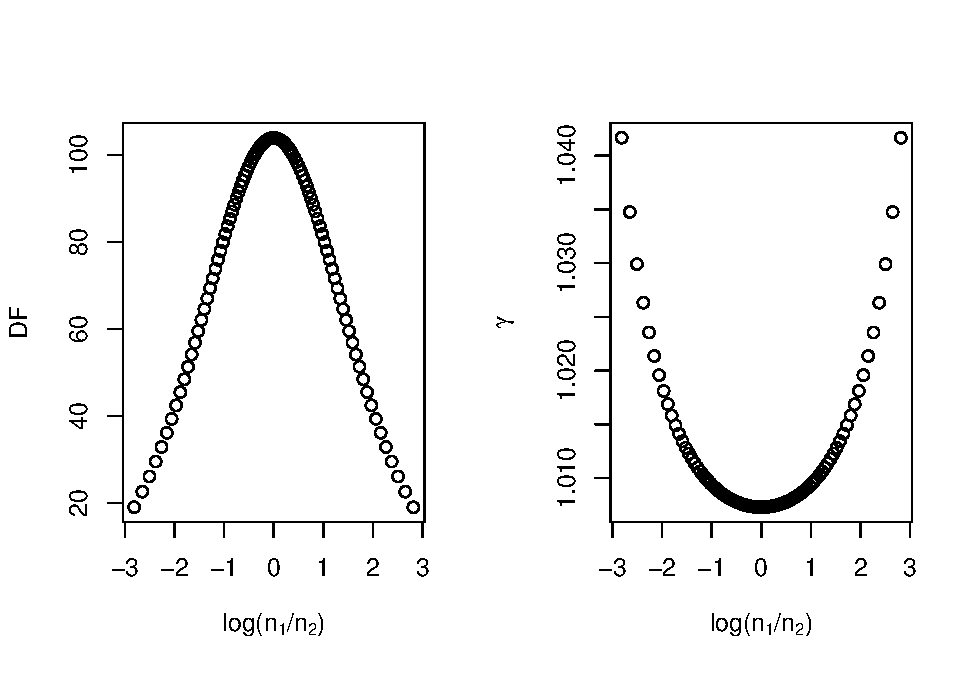
\includegraphics{Theoretical-Bias-of-all-estimators-as-a-function-of-population-parameters_files/figure-latex/biasshiehhetunbalSDRNandnpairing2case1-1.pdf}
\caption{\label{fig:biasshiehhetunbalSDRNandnpairing2case1}\ldots{}}
\end{figure}

\begin{figure}
\centering
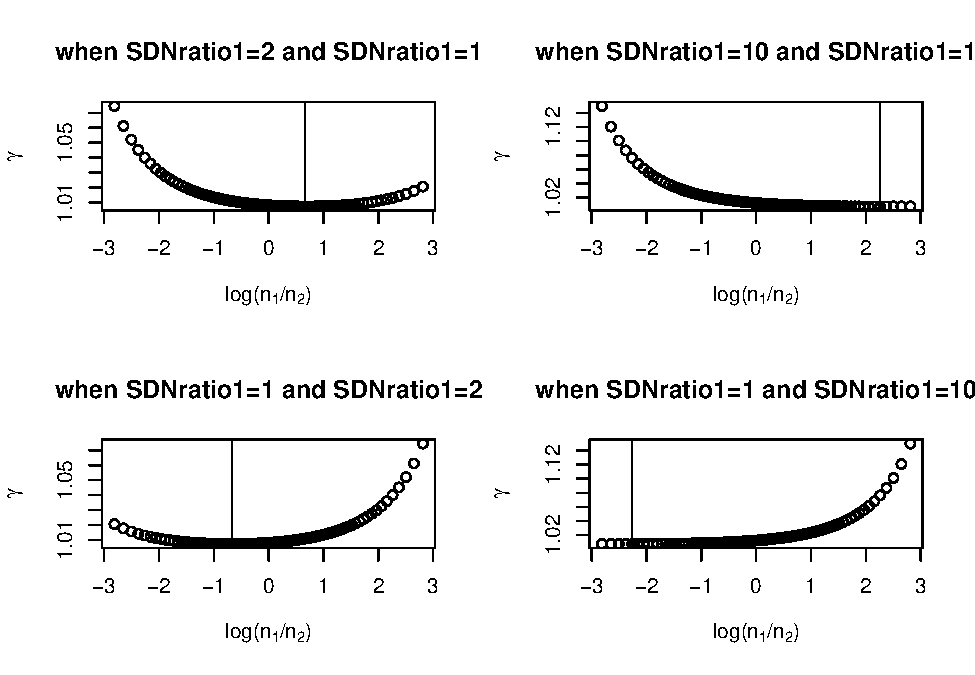
\includegraphics{Theoretical-Bias-of-all-estimators-as-a-function-of-population-parameters_files/figure-latex/biasshiehhetunbalSDRNandnpairing2case2-1.pdf}
\caption{\label{fig:biasshiehhetunbalSDRNandnpairing2case2}\ldots{}}
\end{figure}

\begin{itemize}
\tightlist
\item
  The variances and sample sizes ratios don't matter per se (see Figure \ref{fig:biasshiehhetunbalSDRN2}). However, the pairing between these ratios and sample sizes has an effect on the bias:

  \begin{itemize}
  \tightlist
  \item
    When \(\frac{\sigma^2_1}{n_1}=\frac{\sigma^2_2}{n_2}\), the smallest bias occurs when sample sizes are equal across groups. The further the sample sizes ratio is from 1, the larger the bias (see Figure \ref{fig:biasshiehhetunbalSDRNandnpairing2case1}).
  \item
    When \(\frac{\sigma^2_1}{n_1} \neq \frac{\sigma^2_2}{n_2}\), the minimum bias will always occure when \(min(\frac{\sigma^2_j}{n_j})\) will be associated with \(min(n_j)\). In other word, when \(\frac{\sigma^2_1}{n_1}>\frac{\sigma^2_2}{n_2}\), the sample sizes ratio associated with the minimum bias will be positive, meaning that \(n_1>n_2\) (and the larger the difference between \(\frac{\sigma^2_1}{n_1}\) and \(\frac{\sigma^2_2}{n_2}\), the further from 1 will be this sample sizes ratio; see the two top plots in Figure \ref{fig:biasshiehhetunbalSDRNandnpairing2case2}). On the other side, when \(\frac{\sigma^2_1}{n_1}<\frac{\sigma^2_2}{n_2}\), the sample sizes ratio associated with the minimum bias will be negative, meaning that \(n_1<n_2\) (and the larger the difference between \(\frac{\sigma^2_1}{n_1}\) and \(\frac{\sigma^2_2}{n_2}\), the further from 1 will be this sample sizes ratio; see the two bottom plots in Figure \ref{fig:biasshiehhetunbalSDRNandnpairing2case2}).
  \end{itemize}
\end{itemize}

\begin{figure}
\centering
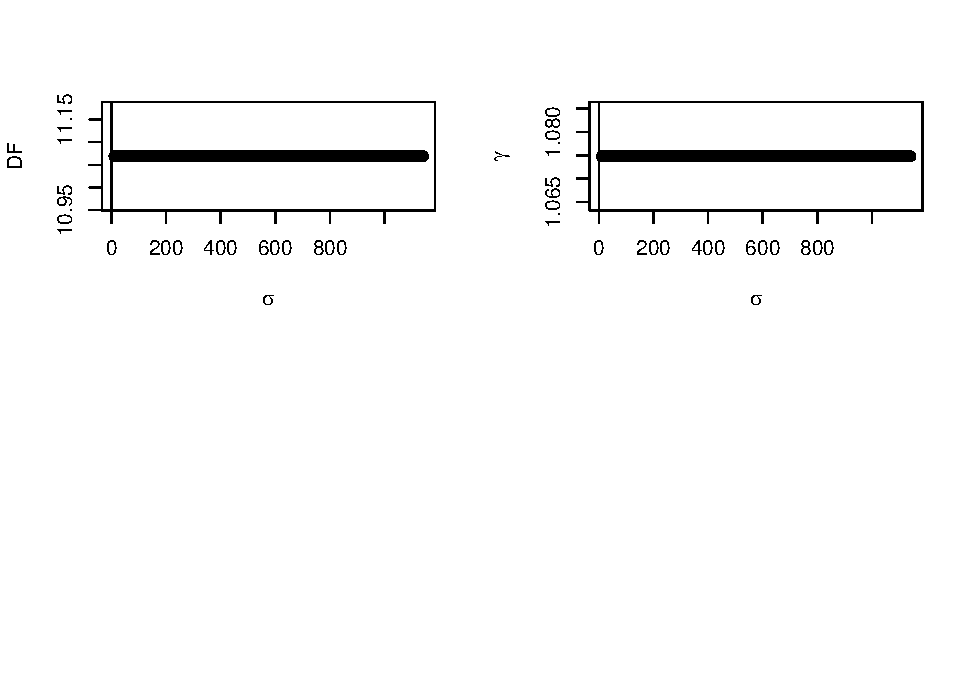
\includegraphics{Theoretical-Bias-of-all-estimators-as-a-function-of-population-parameters_files/figure-latex/biasshiehhetunbalvariance2-1.pdf}
\caption{\label{fig:biasshiehhetunbalvariance2}\ldots{}}
\end{figure}

Moreover, for a constant SD-ratio, the variances don't matter either. (See Figure \ref{fig:biasshiehhetunbalvariance2})

\end{document}
